\section{Results}\label{sec:results}

% Every number in this section comes from a run directory (results/pesquisa/...) with a manifest.
% Validation-pilot numbers are labeled as such and will be replaced by closed-test numbers.

\subsection{Why pruning is not enough}\label{sec:res-pruning}
On the 32 validation instances, the GNN ranked facilities better than the classical service-ratio
score (AUC 0.947--0.950 over three seeds, against 0.905), and adding LP features raised it to
0.959. Ranking quality did not translate into safe pruning. Figure~\ref{fig:rho} shows the
fraction of instances whose restricted problem still contains every facility of the best known
solution as a function of the kept fraction. The LP relaxation, with no training, is above the GNN
for kept fractions from 0.2 to 0.7. To contain the best solution in 80\% of the instances, both
require keeping about 80\% of the facilities. The feasibility repair alone keeps at least 41\%,
because capacity requires slack.

\begin{figure}[t]\centering
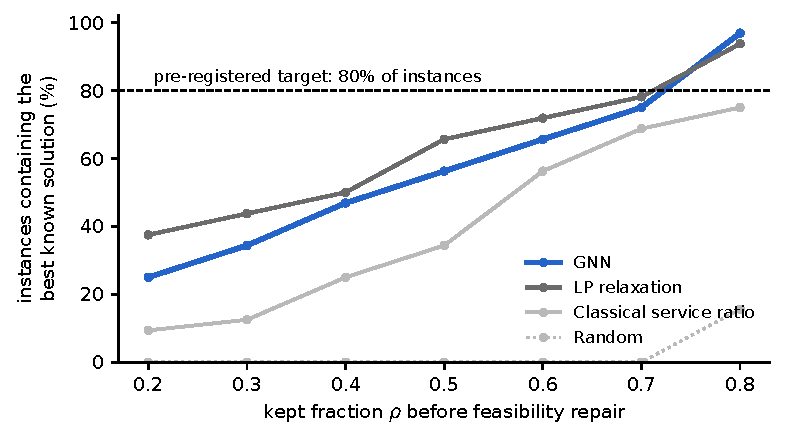
\includegraphics[width=0.92\linewidth]{../figuras/rho.pdf}
\caption{Pruning safety on the 32 validation instances (30 candidate facilities, 150 customers).
Each ranker orders the facilities; the restricted problem keeps the best-ranked fraction $\rho$
(horizontal axis) and a feasibility repair then adds facilities until a first-fit-decreasing
packing of all demands fits and every customer has one of its five cheapest facilities (the
repair alone keeps at least 41\% of the facilities, so small $\rho$ values do not mean small
restricted problems). The vertical axis is the percentage of instances whose restricted problem
still contains \emph{every} facility open in the best known solution, i.e., the percentage in
which pruning has not excluded that solution; higher is safer. The dashed line is the
pre-registered target of 80\%. \emph{GNN}: bipartite graph neural network of
Section~\ref{sec:gnn} (seed 0). \emph{LP relaxation}: facilities ordered by their opening value
$y_i$ in the strong LP. \emph{Classical service ratio}: $(f_i + \text{cost of serving its cheapest
customers up to } Q_i)$ divided by the served demand, the criterion of the greedy add heuristic.
\emph{Random}: uniform order. Source: \texttt{results/pesquisa/etapa1/rho\_validacao.csv}.}
\label{fig:rho}
\end{figure}

\subsection{Coordination is necessary}\label{sec:res-decomp}
Solving clusters independently (Section~\ref{sec:problem}) produced a capacity-infeasible union
in every examined validation instance, with 690--1{,}070 units of overload; after greedy repair
the solutions were 19--29\% above the reference. In the validation pilot, the naive decomposition
had a primal integral of 0.497 and a median final deviation of 28.8\%, against 0.024--0.041 and
1.2--2.7\% for the coordinated CLNS. The naive decomposition was not
carried to the closed test.

\subsection{Validation pilots (not the closed test)}\label{sec:res-pilot}
A first pilot (16 validation instances, one seed) motivated the hybrid. The adaptive expansion had
the lowest primal integral (0.020) and final deviation (0.3\%). CLNS variants found good solutions
early (primal integral 0.024--0.041, against 0.062--0.074 for SCIP and LNS) but stalled at
1.2--2.7\% above the best. The learned selector was the best CLNS selector but did not separate
from rotation (wins on 62\% of the instances, $p=0.43$). Figure~\ref{fig:pilot1} shows both
metrics.

\begin{figure}[t]\centering
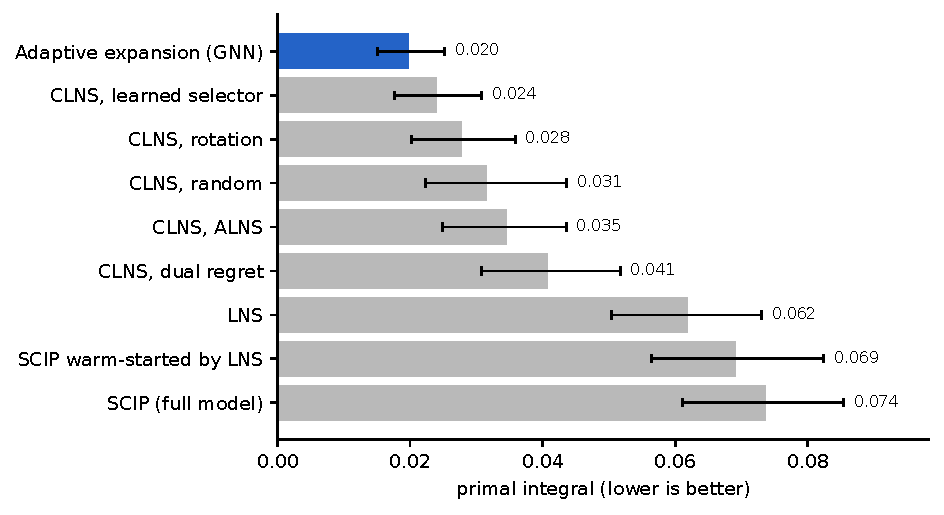
\includegraphics[width=0.49\linewidth]{../figuras/piloto1_integral.pdf}\hfill
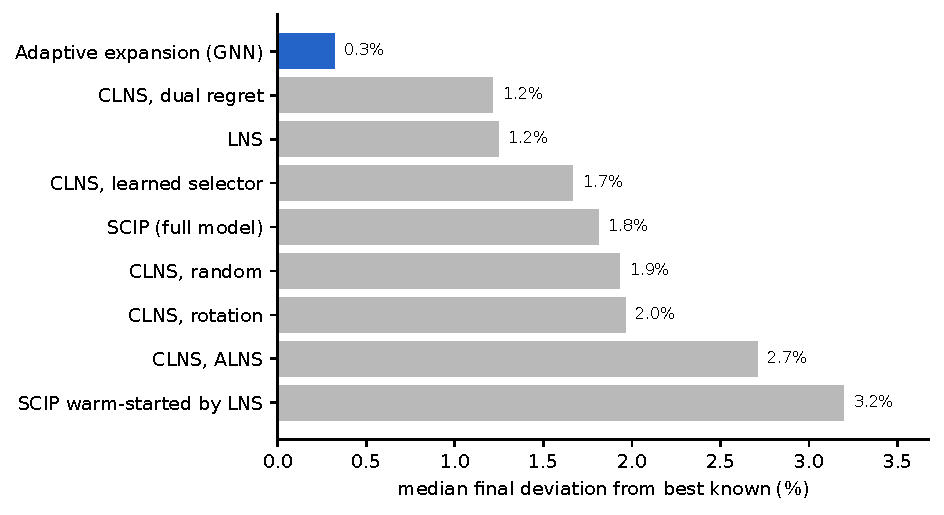
\includegraphics[width=0.49\linewidth]{../figuras/piloto1_desvio.pdf}
\caption{First validation pilot: 16 instances ($30\times150$), budget $T=60$~s, one solver seed
per method. \emph{Left, primal integral} $P = \frac{1}{T}\int_0^T g(t)\,dt$, where
$g(t) = \min\{1, (z^\ast(t) - z_{\mathrm{BKS}})/z_{\mathrm{BKS}}\}$, $z^\ast(t)$ is the best
solution found by time $t$ (with $g(t)=1$ before the first solution) and $z_{\mathrm{BKS}}$ is the
best known cost of the instance (the minimum over all methods and the reference label). $P=0$
means the best known solution was available from time zero; $P=1$ means no solution during the
whole budget. It rewards finding good solutions \emph{early}, not only ending well; lower is
better. Bars are means over instances; whiskers are 95\% bootstrap confidence intervals of the
mean (4{,}000 resamples of instances). \emph{Right, median final deviation}
$(z_{\mathrm{final}} - z_{\mathrm{BKS}})/z_{\mathrm{BKS}}$ at $T$, in percent; lower is better.
The naive decomposition (primal integral 0.497, deviation 28.8\%) is omitted to keep the scale
readable. Highlighted: the method with the lowest primal integral. Source:
\texttt{results/pesquisa/clns/81dbbcb06942419706f3}.}
\label{fig:pilot1}
\end{figure}

\paragraph{Second pilot: the hybrid.} The second pilot used the same 16 instances with three
solver seeds for stochastic methods (432 runs) under the timing protocol of
Section~\ref{sec:protocol}. Two hypotheses were registered beforehand: (H-a) the hybrid with the
GNN-guided selector has a lower primal integral than the adaptive expansion alone; (H-b) inside
the hybrid, the GNN-guided selector beats rotation and the learned selector.
Table~\ref{tab:pilot2} and Figures~\ref{fig:pilot2}--\ref{fig:pilot2-wins} report the outcome.

\begin{table}[t]\centering\small
\caption{Second validation pilot (16 instances, $30\times150$, $T=60$~s; seeds averaged within
instance). $P$: mean primal integral \eqref{eq:pi} with 95\% bootstrap interval; \emph{Dev.}:
median final deviation $g(T)$; $\le1\%$ and $\le0.1\%$: share of instances whose final deviation
is within that tolerance; \emph{Best}: share of instances in which the method has the lowest
final deviation (ties counted for all). Rows sorted by $P$.}\label{tab:pilot2}
\resizebox{\linewidth}{!}{%
\begin{tabular}{lcrrrr}
\toprule
Method & $P$ (95\% CI) & Dev. (\%) & $\le1\%$ & $\le0.1\%$ & Best \\
\midrule
Adaptive expansion (GNN) & 0.0257 (0.019--0.035) & 0.81 & 62.5 & 12.5 & 25.0 \\
Hybrid, learned selector & 0.0270 (0.020--0.036) & 0.57 & 87.5 & 6.3 & 12.5 \\
Hybrid, rotation & 0.0274 (0.021--0.035) & 0.63 & 62.5 & 18.8 & 25.0 \\
CLNS, learned selector & 0.0292 (0.023--0.036) & 2.12 & 12.5 & 0.0 & 6.3 \\
Hybrid, GNN-guided & 0.0296 (0.022--0.040) & 0.62 & 68.8 & 12.5 & 25.0 \\
CLNS, ALNS & 0.0337 (0.029--0.038) & 2.40 & 12.5 & 0.0 & 0.0 \\
CLNS, rotation & 0.0359 (0.030--0.043) & 2.31 & 18.8 & 0.0 & 6.3 \\
CLNS, GNN-guided & 0.0423 (0.034--0.051) & 1.88 & 0.0 & 0.0 & 6.3 \\
LNS & 0.0700 (0.059--0.082) & 1.84 & 12.5 & 0.0 & 0.0 \\
SCIP warm-started by LNS & 0.0705 (0.059--0.084) & 3.59 & 25.0 & 0.0 & 0.0 \\
SCIP (full model) & 0.0795 (0.067--0.091) & 2.66 & 18.8 & 12.5 & 12.5 \\
\bottomrule
\end{tabular}}
\end{table}

Neither hypothesis was supported. (H-a) The adaptive expansion alone has the lowest primal
integral (0.0257); the three hybrids are within its confidence interval (0.0270--0.0296) but not
below it. What the hybrid changes is the \emph{end} of the run: its median final deviation is
0.57--0.63\% against 0.81\%, and with the learned selector 87.5\% of the instances finish within
1\% of the best known solution, against 62.5\%. The anytime curves (Figure~\ref{fig:pilot2},
right) are consistent with this: after $\alpha T=30$~s the expansion flattens near 0.8\%, while
the CLNS phase keeps improving. The two curves need not coincide before $\alpha T$, and they do
not (2.8\% against 3.5\% at 5~s), because the expansion alone allots its stages from a budget of
$T$ and the hybrid from $\alpha T$. The primal integral, dominated by the first seconds, barely
registers the late gain. (H-b) Inside the hybrid, the GNN-guided selector (0.0296) is not better than
rotation (0.0274) or the learned selector (0.0270); the differences are far smaller than the
intervals. The facility scores help in ordering the facilities for the expansion, but once a
good solution exists they carry no measurable information about \emph{where} to search next.

Two further observations hold across both pilots. First, every method that restricts the search
space dominates SCIP on the full model in primal integral by a factor of 2--3, and the hybrids have a lower final deviation in 13--14 of 16 instances (Figure~\ref{fig:pilot2-wins}). Second, CLNS
without the expansion stalls at about 2\%, regardless of the selector: one hypothesis, not tested here, is
that from the LP-rounded solution the improving moves require opening and closing several
facilities at once, which the five neighborhoods rarely free together. This is the motivation for the controls of
Section~\ref{sec:res-controls}: if neither the GNN nor the learned selector separates from its
learning-free counterpart, the gain may come from the mechanisms (nested restriction,
coordinated subproblems) rather than from learning.

\begin{figure}[t]\centering
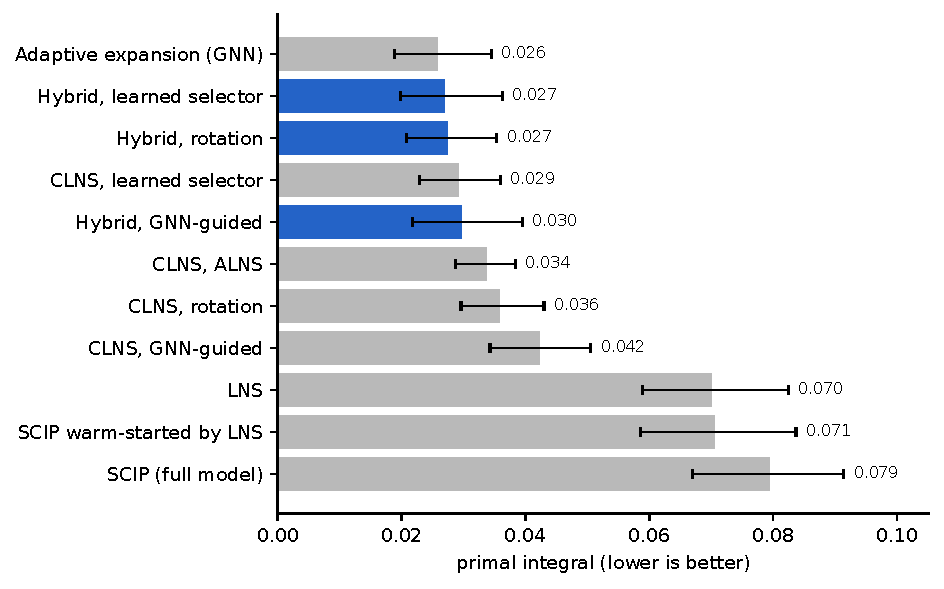
\includegraphics[width=0.49\linewidth]{../figuras/piloto2_integral.pdf}\hfill
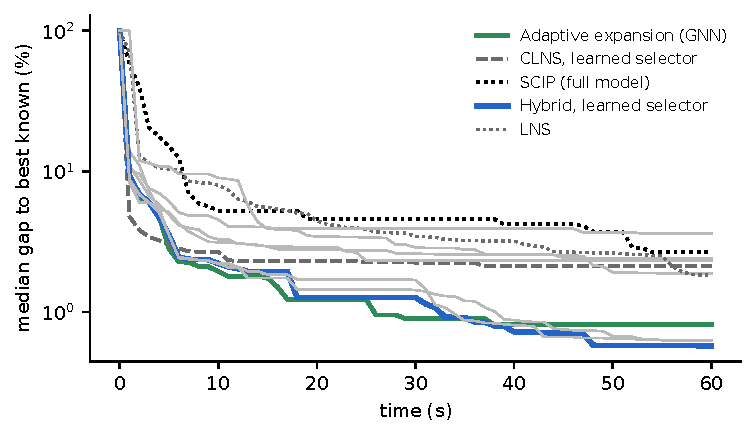
\includegraphics[width=0.49\linewidth]{../figuras/piloto2_anytime.pdf}
\caption{Second validation pilot (16 instances, $30\times150$, $T=60$~s, three seeds averaged
within instance). \emph{Left}: mean primal integral $P$ \eqref{eq:pi} per method; whiskers are
95\% bootstrap confidence intervals over instances; the three hybrids are highlighted; lower is
better. The whiskers are marginal intervals; paired comparisons are given in the text.
\emph{Right}: anytime behaviour. For each second $t$ of the budget, the curve is the median over
instances of the primal gap $g(t)$ in percent (logarithmic vertical axis; a value of $10^0$ is a
1\% gap). A curve that drops early and stays low has a small primal integral; a curve that keeps
dropping late has a small final deviation. Highlighted: hybrid with the learned selector (blue),
adaptive expansion (green), CLNS with the learned selector (dashed), SCIP on the full model
(dotted black) and LNS (dotted grey); the remaining methods are drawn in light grey for context.
Source: \texttt{results/pesquisa/clns/eaa3f86d9312c0970ce9/agregados.json}.}
\label{fig:pilot2}
\end{figure}

\begin{figure}[t]\centering
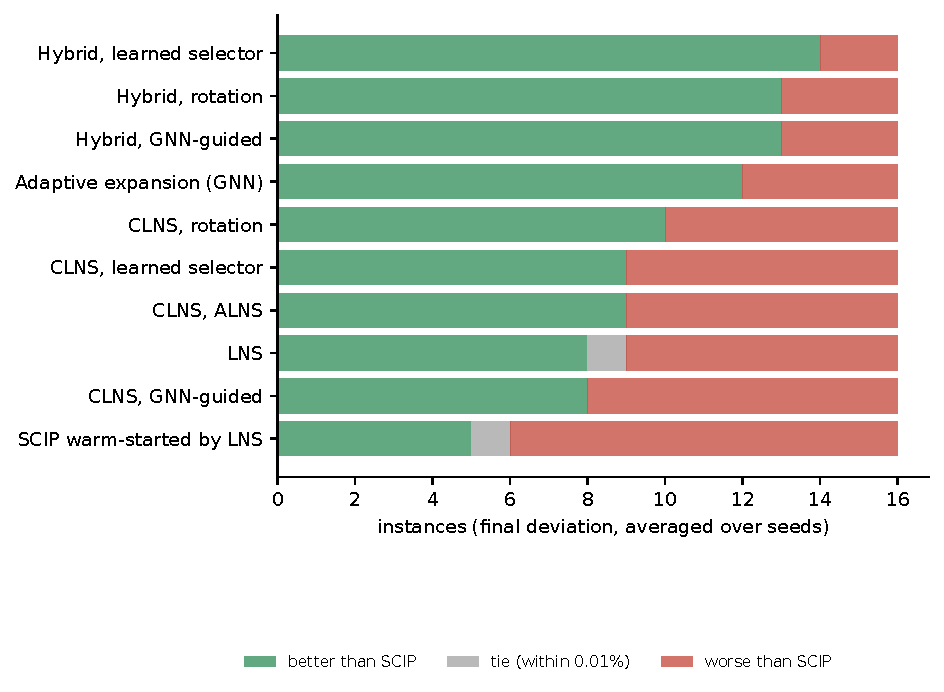
\includegraphics[width=0.49\linewidth]{../figuras/piloto2_vitorias.pdf}\hfill
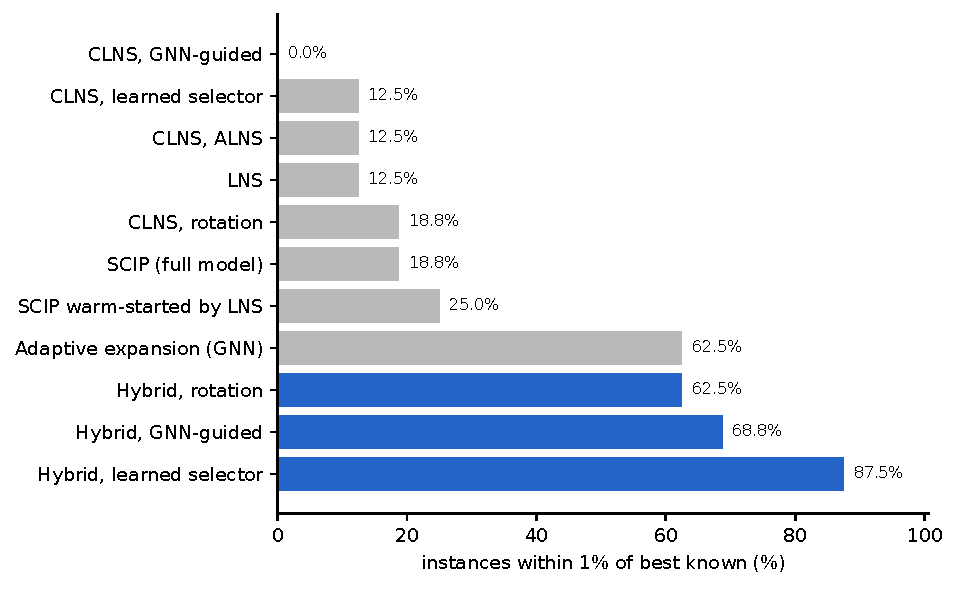
\includegraphics[width=0.49\linewidth]{../figuras/piloto2_ate1pct.pdf}
\caption{Second validation pilot, paired and threshold views. \emph{Left}: for each method, the
number of the 16 instances in which its final deviation (seeds averaged) is lower than
(green), equal within $10^{-4}$ to (grey) or higher than (red) that of SCIP on the full model.
This is a descriptive count; it does not depend on the magnitude of the differences, which the
Wilcoxon test does use. \emph{Right}: percentage of instances whose final deviation is at most 1\%; hybrids
highlighted; higher is better. Same source as Figure~\ref{fig:pilot2}.}
\label{fig:pilot2-wins}
\end{figure}

\subsection{Is learning necessary? Classical controls and subproblem memory}\label{sec:res-controls}
The third pilot used the same 16 validation instances, budget and protocol (352 runs), with the
corrected CLNS code, and added the learning-free controls of Sections~\ref{sec:expansion} and
\ref{sec:kernel} and the memory of Section~\ref{sec:memory}. It answers two questions: does the
GNN matter, and does remembering failed subproblems help? Since it re-ran SCIP, the GNN expansion,
CLNS and the hybrid with rotation, it also checks the second pilot under the corrected code: the
picture is unchanged (hybrid and expansion tied, CLNS alone behind them, SCIP last).

\begin{table}[t]\centering\small
\caption{Third validation pilot (16 instances, $30\times150$, $T=60$~s; seeds averaged within
instance). Columns as in Table~\ref{tab:pilot2}. \emph{Learned}: whether any component of the
method was trained. Rows sorted by $P$.}\label{tab:pilot3}
\resizebox{\linewidth}{!}{%
\begin{tabular}{lccrrrr}
\toprule
Method & Learned & $P$ (95\% CI) & Dev. (\%) & $\le1\%$ & $\le0.1\%$ & Best \\
\midrule
Adaptive expansion (LP) & no & 0.0192 (0.015--0.024) & 0.17 & 56.3 & 43.8 & 31.3 \\
LP hybrid, rotation & no & 0.0215 (0.017--0.026) & 0.53 & 75.0 & 18.8 & 31.3 \\
LP hybrid, rotation + memory & no & 0.0217 (0.017--0.027) & 0.59 & 87.5 & 18.8 & 31.3 \\
Hybrid (GNN), rotation & yes & 0.0236 (0.019--0.028) & 0.87 & 68.8 & 12.5 & 6.3 \\
Hybrid (GNN), rotation + memory & yes & 0.0238 (0.019--0.029) & 0.87 & 68.8 & 12.5 & 12.5 \\
Adaptive expansion (GNN) & yes & 0.0240 (0.018--0.030) & 0.93 & 50.0 & 12.5 & 12.5 \\
Kernel search & no & 0.0258 (0.019--0.033) & 0.99 & 56.3 & 12.5 & 18.8 \\
CLNS, rotation + memory & no & 0.0347 (0.031--0.039) & 2.36 & 0.0 & 0.0 & 0.0 \\
CLNS, rotation & no & 0.0372 (0.032--0.043) & 2.80 & 0.0 & 0.0 & 0.0 \\
SCIP (full model) & no & 0.0706 (0.060--0.081) & 2.44 & 18.8 & 6.3 & 6.3 \\
\bottomrule
\end{tabular}}
\end{table}

\paragraph{No evidence of a benefit from the GNN.} Replacing the GNN score by the LP score \eqref{eq:lpscore},
which requires no training data, did not worsen any method and numerically improved all of them
(Table~\ref{tab:pilot3}, Figure~\ref{fig:pilot3}). For the adaptive expansion, the LP score gave
a primal integral of 0.0192 against 0.0240 and a median final deviation of 0.17\% against 0.93\%;
it had the lower primal integral in 11 of the 16 instances (paired Wilcoxon $p=0.13$). For the
hybrid, 0.0215 against 0.0236 (lower in 10 of 16, $p=0.43$). With 16 instances none of these
differences is significant, so the supported statement is the weaker one: \emph{there is no
evidence that the learned score helps}, and the point estimates favor the learning-free score.
This is consistent with Section~\ref{sec:res-pruning}, where the LP ranking was at least as safe
as the GNN for pruning. Kernel search, the established classical method, is at the level of the
GNN expansion (0.0258 against 0.0240; $p=0.16$ against the LP expansion) and beats SCIP on the
full model in 14 of 16 instances. The reduced-cost certificate \eqref{eq:cert} closed one of the
16 instances before the last stage for both scores.

\paragraph{What the CLNS phase adds.} With the LP score, the hybrid does not improve the primal
integral of the expansion alone (0.0215 against 0.0192, $p=0.40$). Its effect on the end of the
run is mixed: more instances finish within 1\% (75.0\% against 56.3\%) and the mean final
deviation is lower by 0.16 percentage points, but fewer finish within 0.1\% (18.8\% against
43.8\%) and the median deviation is higher (0.53\% against 0.17\%). The expansion, given the
whole budget, closes or nearly closes the easier instances; the hybrid, which stops the
expansion at $\alpha T$, trades those for more robust results on the harder ones. The choice of
$\alpha$ therefore matters and is part of the ablations.

\paragraph{Subproblem repetition and memory.} Without memory, 54--58\% of the subproblems
selected by the CLNS had already failed from the same local state with at least the same time
limit (Figure~\ref{fig:pilot3-mem}): more than half of the iterations re-ran a mixed-integer
program that had already been tried without success under at least the same limit. Memory removed about half of these; the remaining
25--27\% are iterations in which \emph{every} generated candidate had already failed under the
current limit. This is not a certificate of local optimality: the subproblems were interrupted,
not solved, and the candidate list is a sample of the neighborhoods. The time freed by memory did
not translate into a measurable gain: for CLNS alone the primal integral went from 0.0372 to
0.0347 ($p=0.18$) and the median deviation from 2.80\% to 2.36\% ($p=0.12$); inside the hybrids
there was no change (differences below 0.0003 in $P$). One reading, compatible with these data but not established by them, is that the CLNS is limited
by the \emph{reach} of its neighborhoods (or by the ten-facility candidate restriction, or by the
short limits) more than by the order in which they are tried. Re-solving a sample of repeated
subproblems with larger limits would separate these explanations and is listed as future work.

\begin{figure}[t]\centering
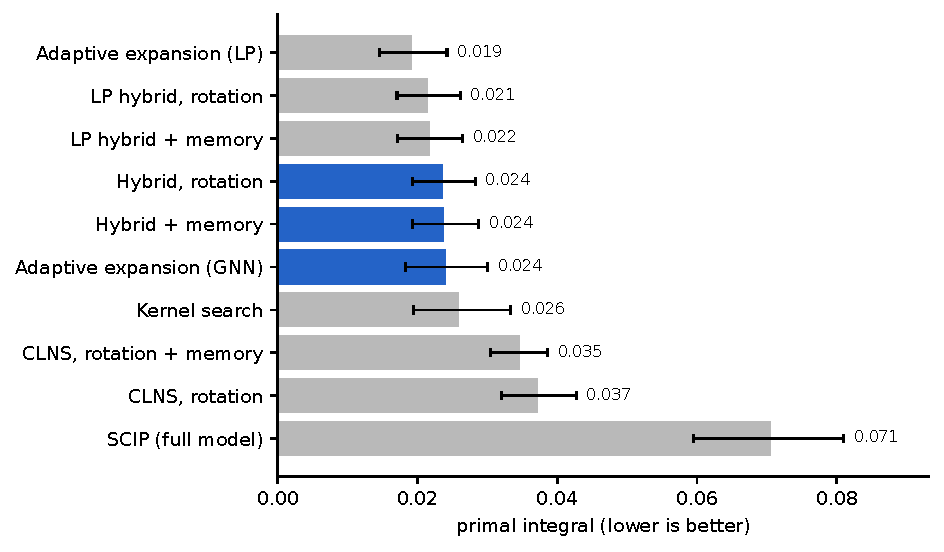
\includegraphics[width=0.49\linewidth]{../figuras/piloto3_integral.pdf}\hfill
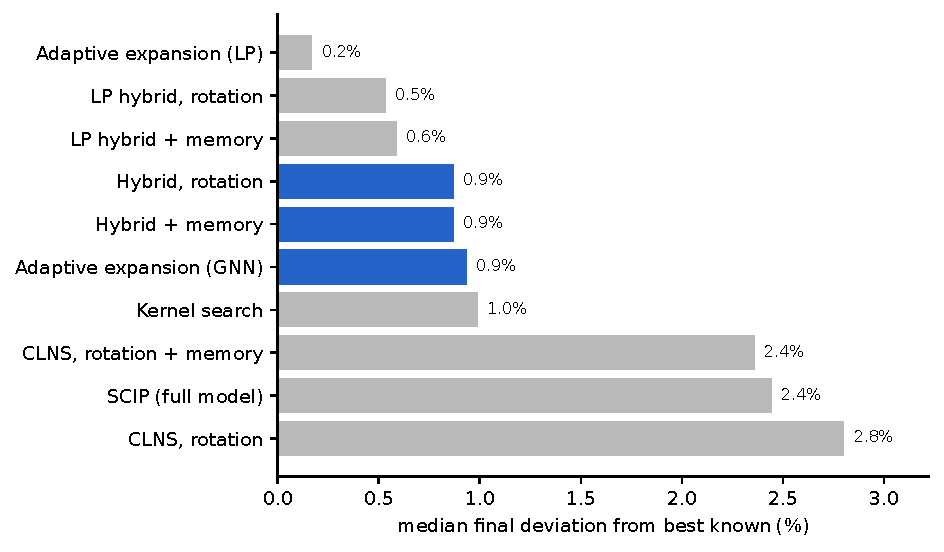
\includegraphics[width=0.49\linewidth]{../figuras/piloto3_desvio.pdf}
\caption{Third validation pilot (16 instances, $30\times150$, $T=60$~s; seeds averaged within
instance). \emph{Left}: mean primal integral $P$ \eqref{eq:pi}; whiskers are 95\% bootstrap
confidence intervals over instances. \emph{Right}: median final deviation $g(T)$ in percent. In
both panels lower is better and the highlighted bars are the methods with a learned component
(the GNN score); grey bars use no training. ``LP'' denotes the score \eqref{eq:lpscore} computed
from the strong LP relaxation. Source:
\texttt{results/pesquisa/clns/e1a72d506f53ea707aa1/agregados.json}.}
\label{fig:pilot3}
\end{figure}

\begin{figure}[t]\centering
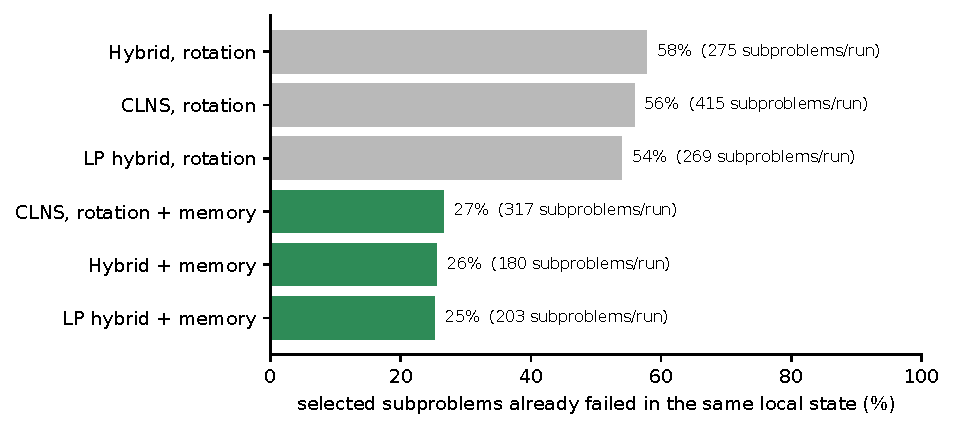
\includegraphics[width=0.7\linewidth]{../figuras/piloto3_repeticao.pdf}
\caption{Repetition of subproblems in the third pilot. For each CLNS variant, the bar is the
percentage of iterations in which the selected subproblem had the same key \eqref{eq:key} as a
subproblem that had already failed to improve with a time limit at least as large, averaged over
seeds and then over instances. Green bars have the memory enabled; for them the remaining
repetitions are iterations in which all candidates were exhausted. The label gives the mean
number of subproblems solved per run; with memory it is lower, plausibly because the subproblems
that remain are those the solver has not yet answered, which take longer. Source:
\texttt{results/pesquisa/clns/e1a72d506f53ea707aa1/resultados.csv}.}
\label{fig:pilot3-mem}
\end{figure}

\paragraph{Measurement.} In this pilot the median CPU/wall ratio was 0.999 and seven of the 352
runs (2.0\%) were below 0.9, all on the same core; the 95th percentile of the budget overrun was
0.04~s.

\subsection{Closed test}\label{sec:res-test}
The closed test was pre-registered after the third pilot and before any run on the instances
below: the six methods, the budgets, four hypotheses and the analysis script were committed
first. It comprises 1{,}390 runs on 139 instances that no pilot had used. The hypotheses are
evaluated on the 64 synthetic instances (test, corridor and scale) with the paired Wilcoxon
signed-rank test and Holm's correction over the four hypotheses, separately for the primal
integral (primary) and the final deviation (secondary):
\begin{description}
\item[H1] restriction helps: the LP-ranked adaptive expansion differs from SCIP on the full model;
\item[H2] learning: the GNN-ranked expansion differs from the LP-ranked expansion;
\item[H3] the CLNS phase: the LP hybrid differs from the LP-ranked expansion alone;
\item[H4] the established classical method: the LP-ranked expansion differs from kernel search.
\end{description}

\begin{table}[t]\centering\small
\caption{Closed test, synthetic sets. $P$: mean primal integral \eqref{eq:pi} with 95\% bootstrap
interval over instances; \emph{Dev.}: median final deviation $g(T)$ from the best known solution;
$\le1\%$: share of instances finishing within 1\%; \emph{W/T/L}: instances in which the final
deviation is lower than, equal to (within $10^{-4}$) or higher than that of SCIP on the full
model. Seeds averaged within instance. Rows sorted by $P$ on the pooled set.}\label{tab:closed}
\resizebox{\linewidth}{!}{%
\begin{tabular}{l rr rr rr | crrc}
\toprule
 & \multicolumn{2}{c}{Test (32, 60 s)} & \multicolumn{2}{c}{Corridor (16, 60 s)} &
 \multicolumn{2}{c|}{Scale (16, 120 s)} & \multicolumn{4}{c}{Pooled (64)} \\
Method & $P$ & Dev. & $P$ & Dev. & $P$ & Dev. & $P$ (95\% CI) & Dev. & $\le1\%$ & W/T/L \\
\midrule
LP hybrid & 0.0385 & 0.35 & 0.0289 & 0.23 & 0.0621 & 0.58 & 0.0420 (0.032--0.053) & 0.35 & 70.3 & 54/3/7 \\
Kernel search & 0.0364 & 0.81 & 0.0341 & 0.85 & 0.0616 & 0.52 & 0.0422 (0.032--0.055) & 0.74 & 57.8 & 46/6/12 \\
Adaptive expansion (LP) & 0.0412 & 0.29 & 0.0311 & 0.73 & 0.0854 & 0.44 & 0.0497 (0.033--0.070) & 0.50 & 65.6 & 50/7/7 \\
Hybrid (GNN) & 0.0506 & 0.55 & 0.0423 & 0.18 & 0.1275 & 2.19 & 0.0677 (0.051--0.087) & 0.62 & 59.4 & 53/3/8 \\
Adaptive expansion (GNN) & 0.0659 & 0.90 & 0.0540 & 0.15 & 0.1699 & 2.03 & 0.0889 (0.058--0.124) & 0.64 & 56.3 & 42/9/13 \\
SCIP (full model) & 0.0794 & 3.21 & 0.1057 & 3.59 & 0.1688 & 7.00 & 0.1083 (0.093--0.124) & 3.72 & 23.4 & -- \\
\bottomrule
\end{tabular}}
\end{table}

\begin{table}[t]\centering\small
\caption{Pre-registered hypotheses on the pooled synthetic set (64 instances). $\bar\Delta$: mean
of the per-instance difference A~$-$~B, with 95\% bootstrap interval; negative values favor A.
The deviation is in percentage points. \emph{A/B}: number of instances in which A or B is
better. $p$: paired Wilcoxon signed-rank test; $p_{\mathrm{Holm}}$: after Holm's correction over
the four hypotheses of the same metric.}\label{tab:hyp}
\resizebox{\linewidth}{!}{%
\begin{tabular}{lll rcrr rcrr}
\toprule
 & & & \multicolumn{4}{c}{Primal integral} & \multicolumn{4}{c}{Final deviation (p.p.)} \\
 & A & B & $\bar\Delta$ (95\% CI) & A/B & $p$ & $p_{\mathrm{Holm}}$ & $\bar\Delta$ (95\% CI) & A/B & $p$ & $p_{\mathrm{Holm}}$ \\
\midrule
H1 & expansion (LP) & SCIP & $-0.059$ ($-0.084$, $-0.031$) & 55/9 & $<0.001$ & $<0.001$ & $-3.10$ ($-4.07$, $-2.18$) & 50/7 & $<0.001$ & $<0.001$ \\
H2 & expansion (GNN) & expansion (LP) & $+0.039$ ($+0.014$, $+0.071$) & 22/42 & 0.001 & 0.004 & $+0.57$ ($+0.14$, $+1.05$) & 15/32 & 0.014 & 0.043 \\
H3 & LP hybrid & expansion (LP) & $-0.008$ ($-0.018$, $+0.001$) & 31/33 & 0.659 & 0.659 & $-0.54$ ($-1.06$, $-0.12$) & 38/19 & 0.025 & 0.050 \\
H4 & expansion (LP) & kernel search & $+0.008$ ($-0.001$, $+0.018$) & 36/28 & 0.319 & 0.638 & $-0.32$ ($-0.69$, $+0.03$) & 33/20 & 0.050 & 0.050 \\
\bottomrule
\end{tabular}}
\end{table}

Tables~\ref{tab:closed} and~\ref{tab:hyp} and Figures~\ref{fig:closed}--\ref{fig:closed-hyp}
give the outcome.

\paragraph{H1: restriction helps.} The LP-ranked expansion has less than half the primal integral
of SCIP on the full model (0.050 against 0.108) and a median final deviation of 0.50\% against
3.72\%; it is better in 55 of the 64 instances ($p_{\mathrm{Holm}}<0.001$ for both metrics).
Every restriction-based method beats the full model in at least 42 instances.

\paragraph{H2: the learned ranking is worse than the LP ranking.} The pilots could only say that
there was no evidence in favor of the GNN. The closed test is stronger: with the GNN in place of
the LP score, the primal integral of the expansion rises from 0.050 to 0.089
($\bar\Delta=+0.039$, interval $+0.014$ to $+0.071$, LP better in 42 of 64,
$p_{\mathrm{Holm}}=0.004$) and the mean final deviation rises by 0.57 percentage points
($p_{\mathrm{Holm}}=0.043$). The loss grows with the distance from the training distribution: on
the scale set, twice as large as anything the GNN was trained on, the GNN-ranked expansion
(0.170) is no better than SCIP on the full model (0.169), whereas the LP-ranked one stays at
0.085. On the corridor family, never seen in training, the GNN variants end with the lowest
\emph{median} deviations (0.15--0.18\%) but have higher primal integrals than their LP
counterparts, so the learned ranking is not uniformly worse at the end of the run; it is slower
to get there. The LP score needs no training data and adapts to each instance by construction.

\paragraph{H3: the CLNS phase improves where the search ends, not how fast it gets there.}
Adding the CLNS phase to the LP-ranked expansion leaves the primal integral unchanged (0.042
against 0.050, $p_{\mathrm{Holm}}=0.66$) and lowers the final deviation by 0.54 percentage
points on average (interval $-1.06$ to $-0.12$; better in 38 instances, worse in 19). The
corrected $p$-value is 0.0495, at the threshold, so we regard this as suggestive rather than
established. The hybrid has the lowest pooled primal integral and the highest share of instances
within 1\% (70.3\%).

\paragraph{H4: the nested expansion is at the level of kernel search.} The two do not differ in
primal integral ($p_{\mathrm{Holm}}=0.64$; kernel search is numerically lower, 0.042 against
0.050). In final deviation the expansion is lower by 0.32 points with an interval that includes
zero ($-0.69$ to $+0.03$) and a corrected $p$-value of 0.0495. We do not claim a difference.
Kernel search, published in 2014 and using no learning, has a numerically lower primal
integral than both learned variants (0.042 against 0.068 and 0.089).

\begin{figure}[t]\centering
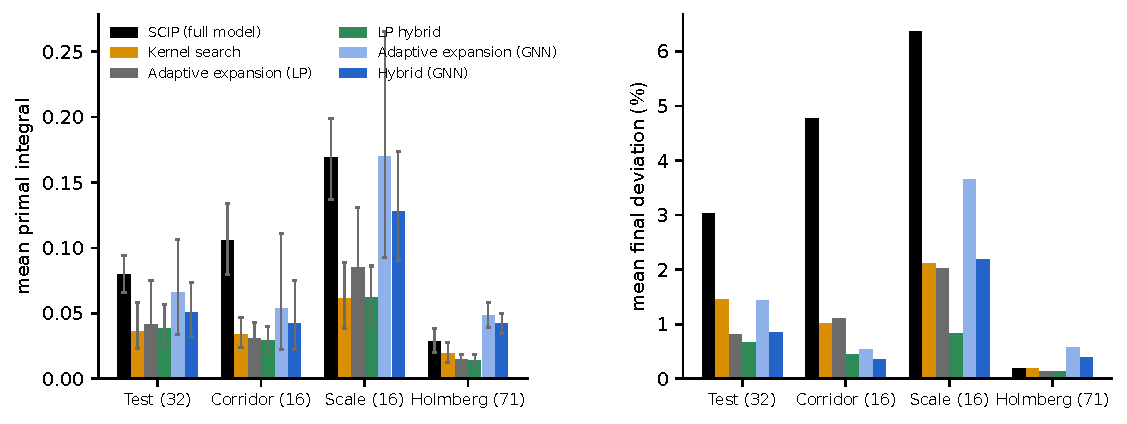
\includegraphics[width=\linewidth]{../figuras/fechado_conjuntos.pdf}
\caption{Closed test, by instance set (number of instances in parentheses). \emph{Left}: mean
primal integral $P$ \eqref{eq:pi}; whiskers are 95\% bootstrap intervals over instances; lower is
better. \emph{Right}: mean final deviation $g(T)$ in percent (from the published optimum for
Holmberg, from the best known solution otherwise). Black: SCIP on the full model. Orange: kernel
search. Grey and green: LP-ranked expansion and LP hybrid, which use no learning. Light and dark
blue: their GNN-ranked counterparts. Within each set the two blue bars are to be compared with the
grey and green ones: the difference is the effect of replacing the LP score by the learned one.
Source: \texttt{results/pesquisa/fechado/analise.json}.}
\label{fig:closed}
\end{figure}

\begin{figure}[t]\centering
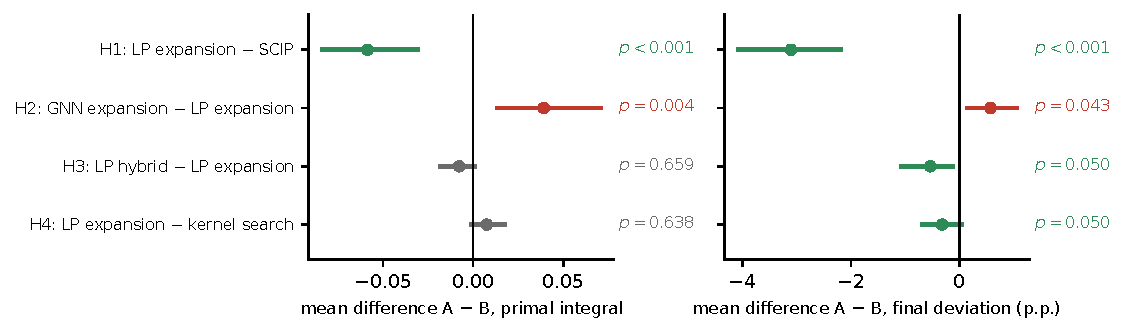
\includegraphics[width=\linewidth]{../figuras/fechado_hipoteses.pdf}
\caption{Pre-registered hypotheses on the 64 pooled synthetic instances. Each row is one paired
comparison A~$-$~B: the dot is the mean per-instance difference and the bar its 95\% bootstrap
interval; a bar entirely to the left of zero means that A is better. \emph{Left}: primal
integral. \emph{Right}: final deviation in percentage points. The value at the right of each row
is the Holm-corrected Wilcoxon $p$-value. Green: significant in favor of A; red: significant in
favor of B; grey: not significant at 0.05.}
\label{fig:closed-hyp}
\end{figure}

\subsection{External anchor: Holmberg instances}\label{sec:res-holmberg}
The 71 Holmberg instances have published optima, so deviations here are true optimality gaps
(Table~\ref{tab:holmberg}). They are small by current standards: SCIP on the full model reaches
the optimum in 61 of them within 30~s, with a median run time of 1.2~s. Three observations hold.
First, the reduced-cost certificate \eqref{eq:cert} works as intended: the expansion stopped with
a \emph{proven} global optimum before its last stage in 59 of the 71 instances, with either
ranking, and with the LP ranking it did so in a median of 0.9~s. Second, the LP-ranked expansion
matches the full model in the number of optima (61) with half its primal integral (0.015 against
0.029). Third, the GNN, trained on Euclidean instances with 30 facilities, transfers poorly to
these non-Euclidean instances: its variants have the highest primal integrals (0.042--0.048),
above the full model, and their certified runs take a median of 4.5~s against 0.9~s, a
difference we attribute to computing the features and the learned score.

\begin{table}[t]\centering\small
\caption{Holmberg instances (71, $T=30$~s). $P$: mean primal integral with 95\% bootstrap
interval; \emph{Mean dev.}: mean deviation from the published optimum; \emph{Optimum}: instances
in which the published optimum was reached (in every seed); \emph{Certified}: instances in which
the expansion proved optimality by reduced costs before its last stage.}\label{tab:holmberg}
\resizebox{\linewidth}{!}{%
\begin{tabular}{lcrrr}
\toprule
Method & $P$ (95\% CI) & Mean dev. (\%) & Optimum & Certified \\
\midrule
LP hybrid & 0.0143 (0.011--0.018) & 0.13 & 59 & -- \\
Adaptive expansion (LP) & 0.0146 (0.011--0.018) & 0.14 & 61 & 59 \\
Kernel search & 0.0191 (0.012--0.028) & 0.18 & 60 & -- \\
SCIP (full model) & 0.0286 (0.020--0.039) & 0.20 & 61 & -- \\
Hybrid (GNN) & 0.0419 (0.035--0.050) & 0.39 & 53 & -- \\
Adaptive expansion (GNN) & 0.0481 (0.039--0.058) & 0.57 & 59 & 59 \\
\bottomrule
\end{tabular}}
\end{table}

\subsection{Case study: Olist}\label{sec:res-olist}
The four real instances grow from $30\times150$ to $150\times850$ and are reported descriptively
(Table~\ref{tab:olist}); four instances support no statistical claim. They show a regime that
the synthetic sets do not reach. On the two largest instances, SCIP on the full model, kernel
search and the expansion alone ended at the same solutions, 8.7--9.3\% above the best known,
and on the largest the expansion returned no feasible solution within 120~s. The hybrids,
whose CLNS phase starts from the LP-rounded solution when the expansion returns nothing, finished
0.02--0.15\% from the best known solution. When the full model no longer fits in the budget,
coordinated decomposition is not a refinement but the only component that makes progress. On the
smallest instance the order is reversed: the full model is already within 0.06\% and the hybrids,
which stop the exact search at $\alpha T$, end slightly behind.

\begin{table}[t]\centering\small
\caption{Olist instances ($T=120$~s): final deviation from the best known solution, in percent,
averaged over seeds. ``--'': no feasible solution within the budget.}\label{tab:olist}
\begin{tabular}{lrrrr}
\toprule
Method & $30\times150$ & $60\times300$ & $100\times600$ & $150\times850$ \\
\midrule
LP hybrid & 0.26 & 1.03 & 0.10 & 0.02 \\
Hybrid (GNN) & 0.19 & 0.73 & 0.15 & 0.02 \\
Kernel search & 0.06 & 0.77 & 8.68 & 9.26 \\
SCIP (full model) & 0.06 & 3.06 & 8.68 & 9.26 \\
Adaptive expansion (LP) & 0.06 & 3.06 & 8.68 & -- \\
Adaptive expansion (GNN) & 0.06 & 3.06 & 8.68 & -- \\
\bottomrule
\end{tabular}
\end{table}

\subsection{Ablations}
\todo{$\alpha\in\{0.3,0.5,0.7\}$; without the opening subproblem; without the LP start; cluster
size 10/15/30.}

\subsection{Measurement quality}\label{sec:res-measure}
Because the comparison is by wall-clock time, a run that waits for the processor is penalized
for reasons unrelated to the algorithm. For every run we record the ratio between the CPU time
of the process and the wall-clock time; a single-threaded run that never waits has ratio 1. In
the 432 runs of the second pilot the median ratio was 0.996 (5th percentile 0.943, 1st percentile
0.911), and three runs (0.7\%) fell below the contention threshold of 0.9
(Figure~\ref{fig:cpu}). The budget overrun, i.e., wall-clock time beyond $T$ caused by
non-preemptible solver calls, had a 95th percentile of 0.075~s and a maximum of 0.82~s
(1.4\% of $T$).

\paragraph{Closed test.} The closed test was less clean than the pilots, and we report it as it
is. Two suspensions of the machine invalidated six runs of the test set (wall-clock times of 646
to 15{,}386~s with a CPU/wall ratio below 0.1); they were discarded by a rule based on time
alone (overrun above 60~s and ratio below 0.1), registered as a deviation before the analysis,
and re-run. More importantly, other workloads were active on the machine during the corridor and
scale sets: the median system load recorded by the harness was 86--91\%, the median CPU/wall
ratio dropped to 0.89 and 0.88, and 187 of their 320 runs fell below the 0.9 threshold. Over
all 1{,}390 runs, 229 (16.5\%) are flagged. The flags are spread over the methods in proportion
to their number of runs, so the contention slows every method rather than a particular one, and
as pre-registered all runs are kept in the main analysis. Repeating the tests of
Table~\ref{tab:hyp} without the flagged runs (38--42 instances remain per comparison) gives the
same conclusions for the primal integral: H1 ($p_{\mathrm{Holm}}<0.001$) and H2
($p_{\mathrm{Holm}}=0.006$) significant, H3 and H4 not ($p_{\mathrm{Holm}}=0.54$). Absolute
primal integrals of the corridor and scale sets should nevertheless be read as upper estimates,
and a replication of these two sets on an idle machine is listed as future work.

\begin{figure}[t]\centering
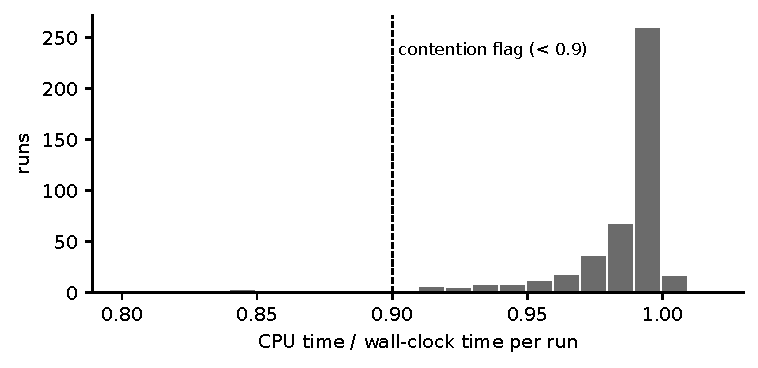
\includegraphics[width=0.7\linewidth]{../figuras/piloto2_cpu_parede.pdf}
\caption{Measurement quality in the second pilot: histogram of the ratio CPU time / wall-clock
time over the 432 runs (bins of 0.01). A ratio of 1 means the process ran without waiting for
the processor; values below the dashed line (0.9) are flagged as suspected contention and
reported, not discarded. The concentration at 0.99--1.00 indicates that pinning each run to a
dedicated physical core removed almost all interference between concurrent runs.}
\label{fig:cpu}
\end{figure}
